{
\newcommand{\myscale}{0.7}
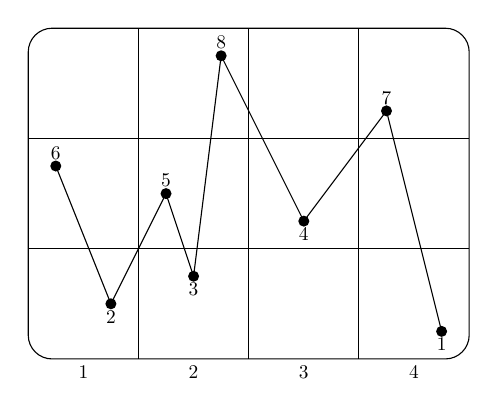
\begin{tikzpicture}[scale=\myscale, every node/.style={scale=\myscale}]
    \draw[rounded corners=2ex] (0,0) rectangle (8,6);
    \foreach \x in {2,4,6} {
        \draw (\x,0) -- (\x,6);
    }
    \foreach \y in {2,4} {
        \draw (0,\y) -- (8, \y);
    }
    \draw (0.5,3.5) -- (1.5,1) -- (2.5,3) -- (3,1.5) -- (3.5,5.5) -- (5,2.5) -- (6.5,4.5) -- (7.5,.5);
    
    \fill (0.5,3.5) circle (0.1) node[above] {$6$};
    \fill (1.5,1) circle (0.1) node[below] {$2$};
    \fill (2.5,3) circle (0.1) node[above] {$5$};
    \fill (3,1.5) circle (0.1) node[below] {$3$};
    \fill (3.5,5.5) circle (0.1) node[above] {$8$};
    \fill (5,2.5) circle (0.1) node[below] {$4$};
    \fill (6.5,4.5) circle (0.1) node[above] {$7$};
    \fill (7.5,.5) circle (0.1) node[below] {$1$};
    \foreach \x in {1,2,3,4} {
        \draw (\x*2-1, 0) node[below] {$\x$};
    }
\end{tikzpicture}
\begin{tikzpicture}[scale=\myscale]
    \draw[white] (0,0) rectangle (2,6);
    \draw[thick, ->] (0,3.4) -- (2,3.4) node[above,pos=.5] {$C_{4312}$};
\end{tikzpicture}
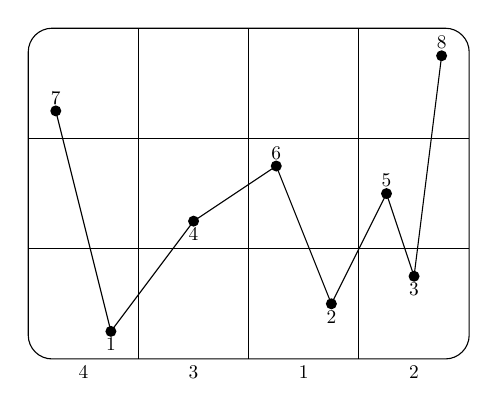
\begin{tikzpicture}[scale=\myscale, every node/.style={scale=\myscale}]
    \draw[rounded corners=2ex] (0,0) rectangle (8,6);
    \foreach \x in {2,4,6} {
        \draw (\x,0) -- (\x,6);
    }
    \foreach \y in {2,4} {
        \draw (0,\y) -- (8, \y);
    }
    \draw (0.5,4.5) -- (1.5,.5) -- (3,2.5) -- (4.5,3.5) -- (5.5,1) -- (6.5,3) -- (7,1.5) -- (7.5,5.5);
    \fill (0.5,4.5) circle (0.1) node[above] {$7$};
    \fill (1.5,.5) circle (0.1) node[below] {$1$};
    \fill (3,2.5) circle (0.1) node[below] {$4$};
    \fill (4.5,3.5) circle (0.1) node[above] {$6$};
    \fill (5.5,1) circle (0.1) node[below] {$2$};
    \fill (6.5,3) circle (0.1) node[above] {$5$};
    \fill (7,1.5) circle (0.1) node[below] {$3$};
    \fill (7.5,5.5) circle (0.1) node[above] {$8$};
    \draw (1,0) node[below] {$4$};
    \draw (3,0) node[below] {$3$};
    \draw (5,0) node[below] {$1$};
    \draw (7,0) node[below] {$2$};
\end{tikzpicture}
}